% Figura cuerpo B3: equivalencia ricardiana en el diagrama de FISHER: la dotación se desliza y el óptimo no se mueve
\documentclass[tikz,border=3pt]{standalone}
\usepackage[T1]{fontenc}
\usepackage[utf8]{inputenc}
\usepackage{amsmath}
\usetikzlibrary{arrows.meta,calc,positioning}
\begin{document}
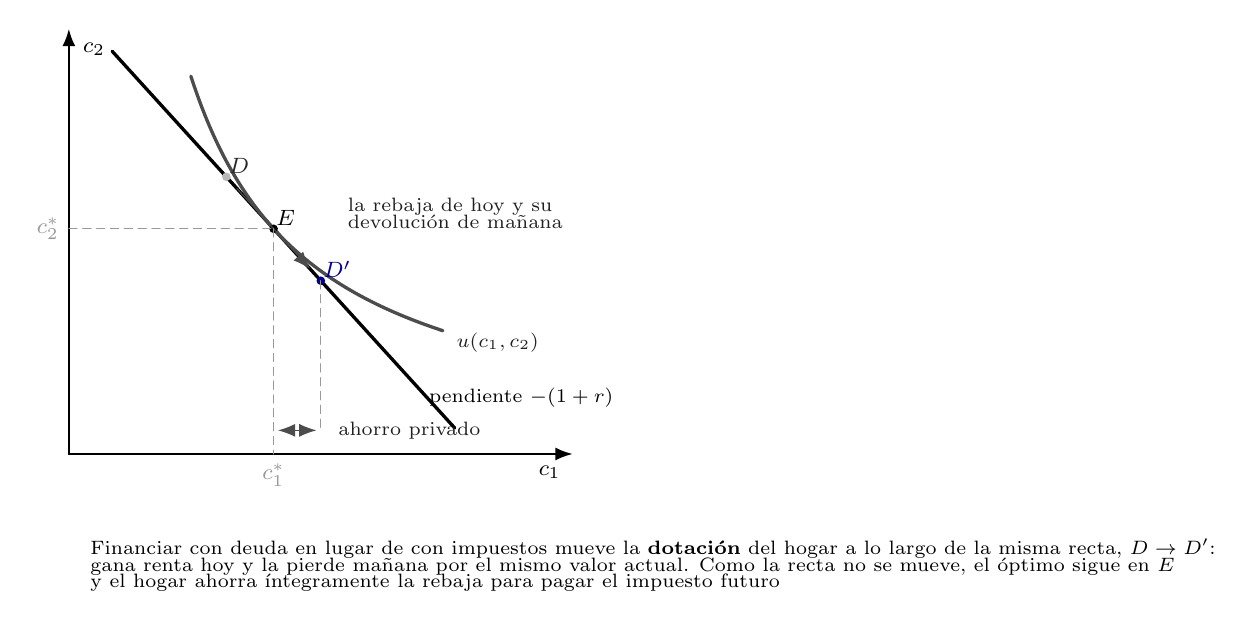
\begin{tikzpicture}[>={Latex[length=2.2mm]}, line cap=round, font=\footnotesize,
  eje/.style={->, thick},
  curva/.style={very thick},
  nueva/.style={very thick, blue!55!black},
  guia/.style={densely dashed, gray!80},
  pto/.style={circle, fill=black, inner sep=1.1pt}]
  \draw[eje] (0,0) -- (6.4,0) node[below left=1pt]{$c_1$};
  \draw[eje] (0,0) -- (0,5.4) node[below right=2pt]{$c_2$};
  % Restriccion presupuestaria intertemporal: c2 = 5.72 - 1.1 c1
  \draw[curva] (0.55,5.115) -- (4.9,0.33);
  \node[anchor=west, font=\scriptsize, align=left] at (4.45,0.72) {pendiente $-(1+r)$};
  % Curva de indiferencia tangente en E: c2 = 7.436/c1
  \draw[curva, gray!60!black, domain=1.55:4.75, samples=70] plot (\x,{7.436/\x});
  \node[anchor=west, font=\scriptsize, text=gray!25!black] at (4.8,1.42) {$u(c_1,c_2)$};
  % Puntos
  \node[pto] (E) at (2.6,2.86) {};
  \node[above right=-2pt of E, inner sep=1pt] {$E$};
  \node[pto, fill=gray!55] (D) at (2.0,3.52) {};
  \node[above right=-2pt of D, inner sep=1pt, gray!30!black] {$D$};
  \node[pto, fill=blue!55!black] (Dp) at (3.2,2.2) {};
  \node[above right=-2pt of Dp, inner sep=1pt, blue!55!black] {$D'$};
  \draw[->, gray!60!black, shorten >=4pt, shorten <=4pt] (D) -- (Dp);
  \node[font=\scriptsize, anchor=west, align=left, text=gray!25!black] at (3.42,3.06)
    {la rebaja de hoy y su\\[-2pt]devolución de mañana};
  \draw[guia] (2.6,2.86) -- (2.6,0) node[below]{$c_1^{*}$};
  \draw[guia] (0,2.86) node[left]{$c_2^{*}$} -- (2.6,2.86);
  % Ahorro nuevo
  \draw[<->, gray!60!black, shorten >=1pt, shorten <=1pt] (2.62,0.3) -- (3.18,0.3);
  \node[font=\scriptsize, anchor=west, text=gray!25!black] at (3.3,0.3) {ahorro privado};
  \draw[guia] (3.2,2.2) -- (3.2,0.3);
  \node[align=left, anchor=north west, font=\scriptsize] at (0.15,-0.95)
    {Financiar con deuda en lugar de con impuestos mueve la \textbf{dotación} del hogar a lo largo de la misma recta, $D\to D'$:\\[-2pt]gana renta hoy y la pierde mañana por el mismo valor actual. Como la recta no se mueve, el óptimo sigue en $E$\\[-2pt]y el hogar ahorra íntegramente la rebaja para pagar el impuesto futuro};
\end{tikzpicture}
\end{document}
